
%% bare_conf.tex
%% V1.4b
%% 2015/08/26
%% by Michael Shell
%% See:
%% http://www.michaelshell.org/
%% for current contact information.
%%
%% This is a skeleton file demonstrating the use of IEEEtran.cls
%% (requires IEEEtran.cls version 1.8b or later) with an IEEE
%% conference paper.
%%
%% Support sites:
%% http://www.michaelshell.org/tex/ieeetran/
%% http://www.ctan.org/pkg/ieeetran
%% and
%% http://www.ieee.org/

%%*************************************************************************
%% Legal Notice:
%% This code is offered as-is without any warranty either expressed or
%% implied; without even the implied warranty of MERCHANTABILITY or
%% FITNESS FOR A PARTICULAR PURPOSE! 
%% User assumes all risk.
%% In no event shall the IEEE or any contributor to this code be liable for
%% any damages or losses, including, but not limited to, incidental,
%% consequential, or any other damages, resulting from the use or misuse
%% of any information contained here.
%%
%% All comments are the opinions of their respective authors and are not
%% necessarily endorsed by the IEEE.
%%
%% This work is distributed under the LaTeX Project Public License (LPPL)
%% ( http://www.latex-project.org/ ) version 1.3, and may be freely used,
%% distributed and modified. A copy of the LPPL, version 1.3, is included
%% in the base LaTeX documentation of all distributions of LaTeX released
%% 2003/12/01 or later.
%% Retain all contribution notices and credits.
%% ** Modified files should be clearly indicated as such, including  **
%% ** renaming them and changing author support contact information. **
%%*************************************************************************


% *** Authors should verify (and, if needed, correct) their LaTeX system  ***
% *** with the testflow diagnostic prior to trusting their LaTeX platform ***
% *** with production work. The IEEE's font choices and paper sizes can   ***
% *** trigger bugs that do not appear when using other class files.       ***                          ***
% The testflow support page is at:
% http://www.michaelshell.org/tex/testflow/



\documentclass[conference]{IEEEtran}
% Some Computer Society conferences also require the compsoc mode option,
% but others use the standard conference format.
%
% If IEEEtran.cls has not been installed into the LaTeX system files,
% manually specify the path to it like:
% \documentclass[conference]{../sty/IEEEtran}





% Some very useful LaTeX packages include:
% (uncomment the ones you want to load)


% *** MISC UTILITY PACKAGES ***
%
%\usepackage{ifpdf}
% Heiko Oberdiek's ifpdf.sty is very useful if you need conditional
% compilation based on whether the output is pdf or dvi.
% usage:
% \ifpdf
%   % pdf code
% \else
%   % dvi code
% \fi
% The latest version of ifpdf.sty can be obtained from:
% http://www.ctan.org/pkg/ifpdf
% Also, note that IEEEtran.cls V1.7 and later provides a builtin
% \ifCLASSINFOpdf conditional that works the same way.
% When switching from latex to pdflatex and vice-versa, the compiler may
% have to be run twice to clear warning/error messages.






% *** CITATION PACKAGES ***
%
%\usepackage{cite}
% cite.sty was written by Donald Arseneau
% V1.6 and later of IEEEtran pre-defines the format of the cite.sty package
% \cite{} output to follow that of the IEEE. Loading the cite package will
% result in citation numbers being automatically sorted and properly
% "compressed/ranged". e.g., [1], [9], [2], [7], [5], [6] without using
% cite.sty will become [1], [2], [5]--[7], [9] using cite.sty. cite.sty's
% \cite will automatically add leading space, if needed. Use cite.sty's
% noadjust option (cite.sty V3.8 and later) if you want to turn this off
% such as if a citation ever needs to be enclosed in parenthesis.
% cite.sty is already installed on most LaTeX systems. Be sure and use
% version 5.0 (2009-03-20) and later if using hyperref.sty.
% The latest version can be obtained at:
% http://www.ctan.org/pkg/cite
% The documentation is contained in the cite.sty file itself.






% *** GRAPHICS RELATED PACKAGES ***
%
\ifCLASSINFOpdf
   \usepackage[pdftex]{graphicx}
  % declare the path(s) where your graphic files are
   \graphicspath{{Figures/}}
  % and their extensions so you won't have to specify these with
  % every instance of \includegraphics
   \DeclareGraphicsExtensions{.pdf,.jpeg,.png}
\else
  % or other class option (dvipsone, dvipdf, if not using dvips). graphicx
  % will default to the driver specified in the system graphics.cfg if no
  % driver is specified.
  % \usepackage[dvips]{graphicx}
  % declare the path(s) where your graphic files are
  % \graphicspath{{../eps/}}
  % and their extensions so you won't have to specify these with
  % every instance of \includegraphics
  % \DeclareGraphicsExtensions{.eps}
\fi
% graphicx was written by David Carlisle and Sebastian Rahtz. It is
% required if you want graphics, photos, etc. graphicx.sty is already
% installed on most LaTeX systems. The latest version and documentation
% can be obtained at: 
% http://www.ctan.org/pkg/graphicx
% Another good source of documentation is "Using Imported Graphics in
% LaTeX2e" by Keith Reckdahl which can be found at:
% http://www.ctan.org/pkg/epslatex
%
% latex, and pdflatex in dvi mode, support graphics in encapsulated
% postscript (.eps) format. pdflatex in pdf mode supports graphics
% in .pdf, .jpeg, .png and .mps (metapost) formats. Users should ensure
% that all non-photo figures use a vector format (.eps, .pdf, .mps) and
% not a bitmapped formats (.jpeg, .png). The IEEE frowns on bitmapped formats
% which can result in "jaggedy"/blurry rendering of lines and letters as
% well as large increases in file sizes.
%
% You can find documentation about the pdfTeX application at:
% http://www.tug.org/applications/pdftex


\usepackage{subfig}


% *** MATH PACKAGES ***
%
%\usepackage{amsmath}
% A popular package from the American Mathematical Society that provides
% many useful and powerful commands for dealing with mathematics.
%
% Note that the amsmath package sets \interdisplaylinepenalty to 10000
% thus preventing page breaks from occurring within multiline equations. Use:
%\interdisplaylinepenalty=2500
% after loading amsmath to restore such page breaks as IEEEtran.cls normally
% does. amsmath.sty is already installed on most LaTeX systems. The latest
% version and documentation can be obtained at:
% http://www.ctan.org/pkg/amsmath





% *** SPECIALIZED LIST PACKAGES ***
%
%\usepackage{algorithmic}
% algorithmic.sty was written by Peter Williams and Rogerio Brito.
% This package provides an algorithmic environment fo describing algorithms.
% You can use the algorithmic environment in-text or within a figure
% environment to provide for a floating algorithm. Do NOT use the algorithm
% floating environment provided by algorithm.sty (by the same authors) or
% algorithm2e.sty (by Christophe Fiorio) as the IEEE does not use dedicated
% algorithm float types and packages that provide these will not provide
% correct IEEE style captions. The latest version and documentation of
% algorithmic.sty can be obtained at:
% http://www.ctan.org/pkg/algorithms
% Also of interest may be the (relatively newer and more customizable)
% algorithmicx.sty package by Szasz Janos:
% http://www.ctan.org/pkg/algorithmicx




% *** ALIGNMENT PACKAGES ***
%
%\usepackage{array}
% Frank Mittelbach's and David Carlisle's array.sty patches and improves
% the standard LaTeX2e array and tabular environments to provide better
% appearance and additional user controls. As the default LaTeX2e table
% generation code is lacking to the point of almost being broken with
% respect to the quality of the end results, all users are strongly
% advised to use an enhanced (at the very least that provided by array.sty)
% set of table tools. array.sty is already installed on most systems. The
% latest version and documentation can be obtained at:
% http://www.ctan.org/pkg/array


% IEEEtran contains the IEEEeqnarray family of commands that can be used to
% generate multiline equations as well as matrices, tables, etc., of high
% quality.




% *** SUBFIGURE PACKAGES ***
%\ifCLASSOPTIONcompsoc
%  \usepackage[caption=false,font=normalsize,labelfont=sf,textfont=sf]{subfig}
%\else
%  \usepackage[caption=false,font=footnotesize]{subfig}
%\fi
% subfig.sty, written by Steven Douglas Cochran, is the modern replacement
% for subfigure.sty, the latter of which is no longer maintained and is
% incompatible with some LaTeX packages including fixltx2e. However,
% subfig.sty requires and automatically loads Axel Sommerfeldt's caption.sty
% which will override IEEEtran.cls' handling of captions and this will result
% in non-IEEE style figure/table captions. To prevent this problem, be sure
% and invoke subfig.sty's "caption=false" package option (available since
% subfig.sty version 1.3, 2005/06/28) as this is will preserve IEEEtran.cls
% handling of captions.
% Note that the Computer Society format requires a larger sans serif font
% than the serif footnote size font used in traditional IEEE formatting
% and thus the need to invoke different subfig.sty package options depending
% on whether compsoc mode has been enabled.
%
% The latest version and documentation of subfig.sty can be obtained at:
% http://www.ctan.org/pkg/subfig




% *** FLOAT PACKAGES ***
%
%\usepackage{fixltx2e}
% fixltx2e, the successor to the earlier fix2col.sty, was written by
% Frank Mittelbach and David Carlisle. This package corrects a few problems
% in the LaTeX2e kernel, the most notable of which is that in current
% LaTeX2e releases, the ordering of single and double column floats is not
% guaranteed to be preserved. Thus, an unpatched LaTeX2e can allow a
% single column figure to be placed prior to an earlier double column
% figure.
% Be aware that LaTeX2e kernels dated 2015 and later have fixltx2e.sty's
% corrections already built into the system in which case a warning will
% be issued if an attempt is made to load fixltx2e.sty as it is no longer
% needed.
% The latest version and documentation can be found at:
% http://www.ctan.org/pkg/fixltx2e


%\usepackage{stfloats}
% stfloats.sty was written by Sigitas Tolusis. This package gives LaTeX2e
% the ability to do double column floats at the bottom of the page as well
% as the top. (e.g., "\begin{figure*}[!b]" is not normally possible in
% LaTeX2e). It also provides a command:
%\fnbelowfloat
% to enable the placement of footnotes below bottom floats (the standard
% LaTeX2e kernel puts them above bottom floats). This is an invasive package
% which rewrites many portions of the LaTeX2e float routines. It may not work
% with other packages that modify the LaTeX2e float routines. The latest
% version and documentation can be obtained at:
% http://www.ctan.org/pkg/stfloats
% Do not use the stfloats baselinefloat ability as the IEEE does not allow
% \baselineskip to stretch. Authors submitting work to the IEEE should note
% that the IEEE rarely uses double column equations and that authors should try
% to avoid such use. Do not be tempted to use the cuted.sty or midfloat.sty
% packages (also by Sigitas Tolusis) as the IEEE does not format its papers in
% such ways.
% Do not attempt to use stfloats with fixltx2e as they are incompatible.
% Instead, use Morten Hogholm'a dblfloatfix which combines the features
% of both fixltx2e and stfloats:
%
% \usepackage{dblfloatfix}
% The latest version can be found at:
% http://www.ctan.org/pkg/dblfloatfix




% *** PDF, URL AND HYPERLINK PACKAGES ***
%
%\usepackage{url}
% url.sty was written by Donald Arseneau. It provides better support for
% handling and breaking URLs. url.sty is already installed on most LaTeX
% systems. The latest version and documentation can be obtained at:
% http://www.ctan.org/pkg/url
% Basically, \url{my_url_here}.




% *** Do not adjust lengths that control margins, column widths, etc. ***
% *** Do not use packages that alter fonts (such as pslatex).         ***
% There should be no need to do such things with IEEEtran.cls V1.6 and later.
% (Unless specifically asked to do so by the journal or conference you plan
% to submit to, of course. )

% correct bad hyphenation here
\hyphenation{op-tical net-works semi-conduc-tor}


\begin{document}
%
% paper title
% Titles are generally capitalized except for words such as a, an, and, as,
% at, but, by, for, in, nor, of, on, or, the, to and up, which are usually
% not capitalized unless they are the first or last word of the title.
% Linebreaks \\ can be used within to get better formatting as desired.
% Do not put math or special symbols in the title.
\title{Bare Demo of IEEEtran.cls\\ for IEEE Conferences}


% author names and affiliations
% use a multiple column layout for up to three different
% affiliations
\author{\IEEEauthorblockN{G. Davila Revelo\\
M. Anderson Ricci\\
J. I. Alvarez-Hamelin}
\IEEEauthorblockA{Facultad de Ingeniería\\
Universidad de Buenos Aires, Argentina\\
Email: ?}}
%\and
%\IEEEauthorblockN{M. Anderson Ricci}
%\IEEEauthorblockA{Facultad de Ingeniería\\
%Universidad de Buenos Aires\\
%Email: ?}
%\and
%\IEEEauthorblockN{J. I. Alvarez-Hamelin}
%\IEEEauthorblockA{Facultad de Ingeniería\\
%Universidad de Buenos Aires\\
%Email: ?}}

% conference papers do not typically use \thanks and this command
% is locked out in conference mode. If really needed, such as for
% the acknowledgment of grants, issue a \IEEEoverridecommandlockouts
% after \documentclass

% for over three affiliations, or if they all won't fit within the width
% of the page, use this alternative format:
% 
%\author{\IEEEauthorblockN{Michael Shell\IEEEauthorrefmark{1},
%Homer Simpson\IEEEauthorrefmark{2},
%James Kirk\IEEEauthorrefmark{3}, 
%Montgomery Scott\IEEEauthorrefmark{3} and
%Eldon Tyrell\IEEEauthorrefmark{4}}
%\IEEEauthorblockA{\IEEEauthorrefmark{1}School of Electrical and Computer Engineering\\
%Georgia Institute of Technology,
%Atlanta, Georgia 30332--0250\\ Email: see http://www.michaelshell.org/contact.html}
%\IEEEauthorblockA{\IEEEauthorrefmark{2}Twentieth Century Fox, Springfield, USA\\
%Email: homer@thesimpsons.com}
%\IEEEauthorblockA{\IEEEauthorrefmark{3}Starfleet Academy, San Francisco, California 96678-2391\\
%Telephone: (800) 555--1212, Fax: (888) 555--1212}
%\IEEEauthorblockA{\IEEEauthorrefmark{4}Tyrell Inc., 123 Replicant Street, Los Angeles, California 90210--4321}}




% use for special paper notices
%\IEEEspecialpapernotice{(Invited Paper)}




% make the title area
\maketitle

% As a general rule, do not put math, special symbols or citations
% in the abstract
\begin{abstract}
The abstract goes here.
\end{abstract}

% no keywords




% For peer review papers, you can put extra information on the cover
% page as needed:
% \ifCLASSOPTIONpeerreview
% \begin{center} \bfseries EDICS Category: 3-BBND \end{center}
% \fi
%
% For peerreview papers, this IEEEtran command inserts a page break and
% creates the second title. It will be ignored for other modes.
\IEEEpeerreviewmaketitle

\section{Introduction}

Internet topology is concerned with the study of the various types of connectivity structures and representations between directly connected nodes in the Internet architecture \cite{Calvert97}. This representations aims to obtain models that represent the Internet with the greatest possible accuracy in order to test new communications protocols, algorithms, QoS policies, traffic engineering, etc. 
 
The first efforts to model the Internet architecture began with Waxman's works in 1988 \cite{Waxman88}. Since there, several sophistication was added to network modelling. The first remarkable characteristic of Internet topology appears  in 1999 [Faloutsos]. It shows that Internet's distribution degree obeys a heavy-tail power law instead of Poison distributed as it was believed. From this discovery, many efforts focused on to get more detailed information about Internet Topology including new metrics and innovations. In this way, it has been shown previously that the k-core decomposition is capable of identifying networks sources by means of the visualization \cite{Alvarez06k} \cite{Beiro09}, may be used to validate models \cite{Serrano06}, and discover exploration biases on the Internet \cite{Alvarez08k}. These facts support the k-core analysis as one of the relevant tools to describe the Internet topology maps. These previous works typically have focused in router level topology and AS level topology, but it does not include details closely related to the current Internet Technologies, i.e, \textit{Multiprotocol Label Switching} clouds. 

MPLS was designed to reduce the time required to make forwarding decision thanks to the insertion of labels before the IP header. It is quite relevant as it commonly deployed in today's Internet \cite{SOM11}, \cite{Donnet12}, \cite{Vanaubel15}.  In this way, we believe that it is necessary to study in more depth MPLS features and its topological properties such as robustness and resilience capability. We turn our attention  in MPLS clouds. First, we validate the accuracy of the signatures that allows to reveal MPLS tunnels. Moreover we build an router level topology where we distinguish \textit{IP links} and \textit{mpls links}. Finally we use the obtained network topology in order to analyse the properties of MPLS networks based on graph analysis tools such as k-core decomposition.


\section{Background}

\subsection{MPLS overview}

Multiprotocol Label Switching (MPLS) \cite{Vanaubel15} was originally designed to speed up the forwarding process. In practice, this was done with one or more 32 bits labelstack entries(LSE) inserted between the frame header  and the IP packet. 

In a MPLS network, packets are forwarded using an exact match lookup of a 20-bit label found in the LSE. An MPLS LSE also has a time-to-live (LSE-TTL) field and a type-of-service field \cite{rfc1771}. At each MPLS hop, the label of the incoming packet is replaced by a corresponding outgoing label found in an MPLS switching table. A portion of a path where the forwarding decision is not anymore based on longest prefix matching but rather on MPLS features is known as an MPLS tunnel. A router with label switching capabilities is called Label Switching Router. 

\subsection{Revealing MPLS tunnels}

MPLS tunnels could be revealed using traceroutes tools based. We can identified two kind of visible MPLS tunnels: explicit tunnels and implicit tunnels.

Explicit tunnels are based on RFC 4950 implementation. MPLS routers may send ICMP time-exceeded messages when the LSE-TTL expires. The RFC 4950 is an extension to ICMP allowing a router to embed an MPLS LSE in an ICMP time-exceeded message. In that case, when the LSE-TTL expires on a MPLS router, it simply quotes the MPLS label stack in the ICMP \texttt{time-exceeded} message. 

Implicit tunnels discovery are based on two signatures: \textit{qttl} signature and\textit{ u-turn} signature. \textit{qttl} signatures are related with \texttt{ttl-propagate} option, if this option is implemented, the first MPLS router (the Ingress Label Edge Router - LER) of an LSP copies the IP-TTL value to the LSE-TTL field rather than setting the LSE-TTL to an arbitrary value, then LSRs along the LSP will reveal themselves via ICMP messages even if they do not implement RFC 4950. Typically the IP packet expires when the TTL value decrease until one ($qttl=1$). Thereby, when $qttl>1$, the ICMP reply message belongs to an MPLS tunnel. U-turn signature relies on the fact that most LSRs in an LSP present a common behavior: when the LSE-TTL expires, the LSR first sends the time-exceeded reply to the LH router which then forwards the reply to the probing source using directly an IP route if available. The difference between these probing messages is identified as \textit{u-turn} signature. These signature on MPLS tunnel discovery are discussing in detail on\cite{Donnet12} . 

The \texttt{qttl} signature ($qttl>1$) is present just in MPLS behaviour. Commonly there is not another way to get a $qttl>1$. However, \texttt{u-turn} signature could be caused for another internet issues such as police routing or load balancing, producing different lengths in the return path. Thereby, in this paper we consider that RFC 4950 implementation and \textit{qttl} signature are highly reliable methods to reveal MPLS tunnels and we mainly focus on to test \texttt{u-turn} signature accuracy.

\subsection{K-core visualization analysis}

The visualization based on {k}-core decomposition is a tool where we can easily read basic features of the graph (Degree, hierarchical structure, etc.) as well as more entangled features, e. g., the relation between a vertex and the hierarchical position of its neighbours. It is also a useful tool to  discriminate between networks with different topological properties and structural arrangement. In this way, we use $k$-core decomposition in order to discriminate between MPLS and IP networks properties. 

Let the graph $G=(V,E)$, \textit{k}-core decomposition analysis is based in the next definitions:

\begin{itemize}
\item[i]{\textbf{\textit{k}-cores}}. A subgraph $H=(C,E|C)$ induced by the set $ C\subseteq V$ is a \textit{k}-core of order $k$ $iff$ $\forall v \in C: degree_{H}(v)\geq k$ and $H$ is the maximum subgraph with this property.

A \textit{k}-core of $G$ can therefore be obtained by recursively removing all the vertices of degree less than $k$, until all vertices in the remaining graph have at least degree $k$. 

\item[ii]\textbf{Shell index}. A vertex $i$ has shell index $c$ if it belongs to the $c$-core but not to $(c+1)$-core. We denote by $C_i$ to the shell index of vertex $i$. A shell $C_c$ is composed by all the vertices whose shell index is $c$. The maximum value $c$ such that $C_c$ is not empty is denoted $C_{max}$. The $k$-core is thus the union of all shells $C_c$ with $c \geq k$.

\end{itemize}

The $k$-core visualization return a two dimensional plot, where the position of each vertex depends on its shell index and on the index of its neighbours. A color code allows for the identification of shell indices, while the vertex’s original degree is provided by its size that depends logarithmically on the degree. A central role in the visualization method is played by multi-components representation of $k$-cores. In the most general situation, indeed, the recursive removal of vertices having degree less than a given $k$ can break the original network into various connected components, each of which might even be once again broken by the subsequent decomposition.

In this work, we use $k$-core decomposition focus on \textit{LSRs} and \textit{mpls clouds} location. So we mainly use the visualization in order to find properties and fingerprints tightly with MPLS presence.


\section{Dataset}

\begin{figure*}[!t]
\centering
\subfloat[Degre Distribution]{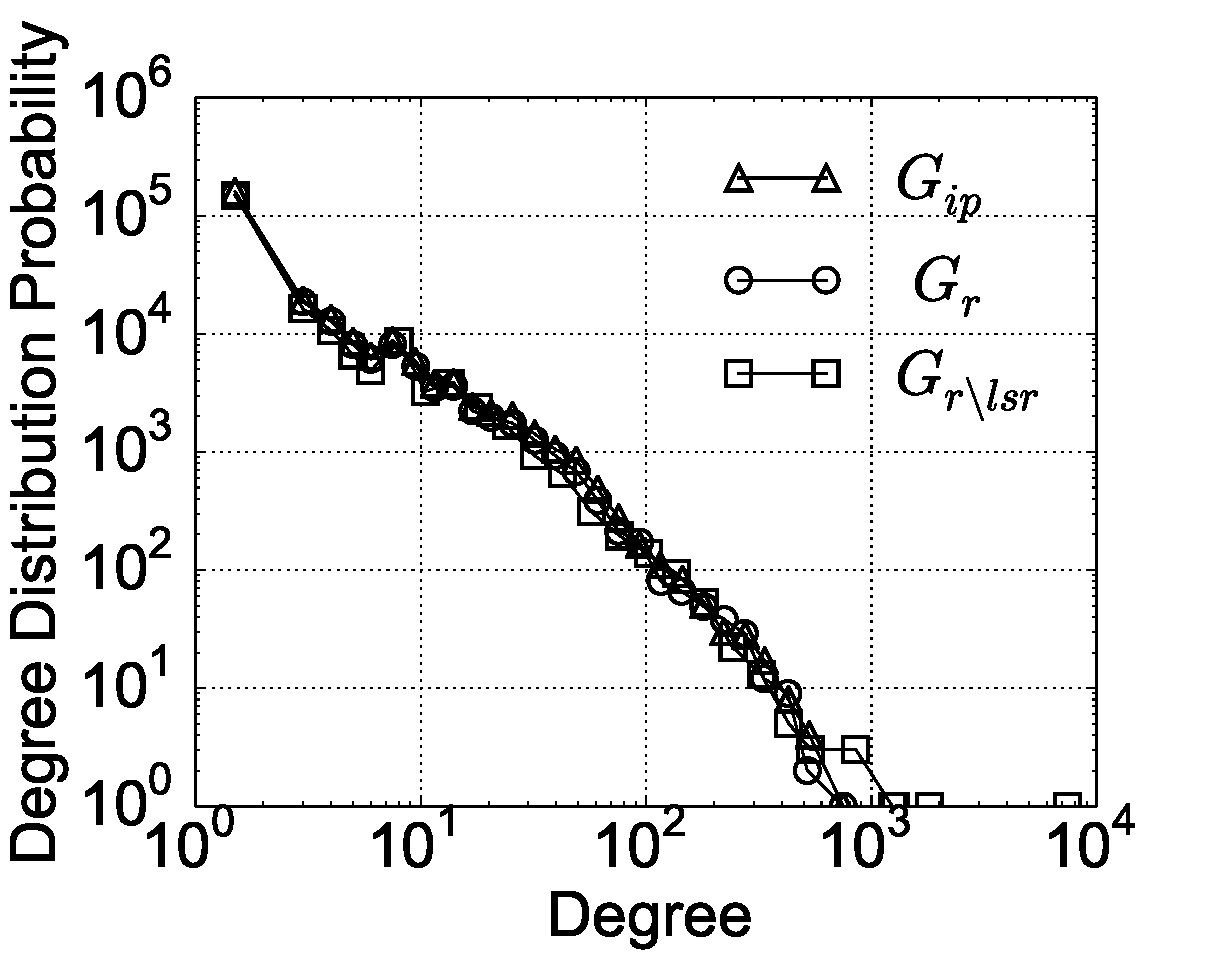
\includegraphics[width=2.2in]{DegreeDistribution}
\label{fig_metrics_a}}
\hfil
\subfloat[Clustering Coeficient]{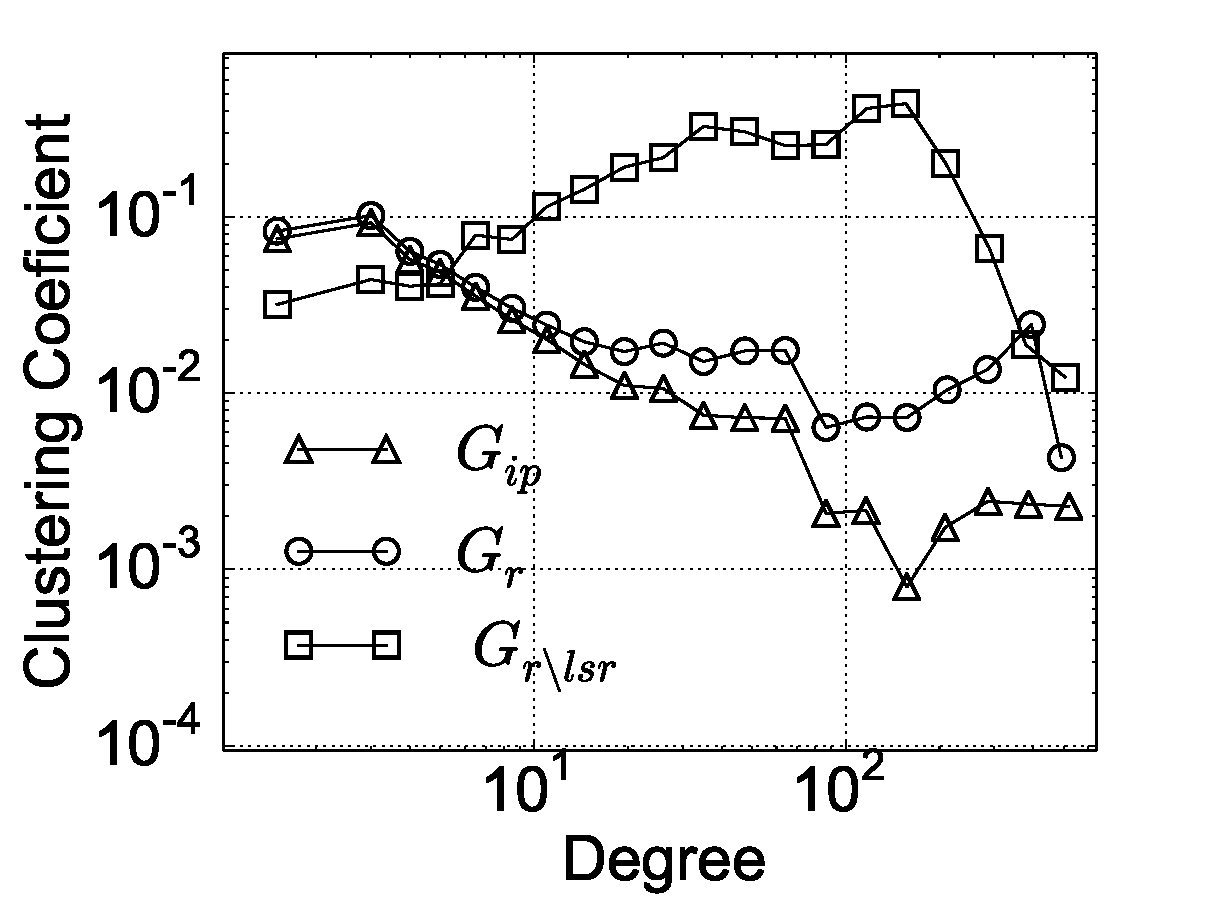
\includegraphics[width=2.2in]{ClusteringCoeficient}
\label{fig_metrics_b}}
\hfil
\subfloat[Neighborg Degree Distribution]{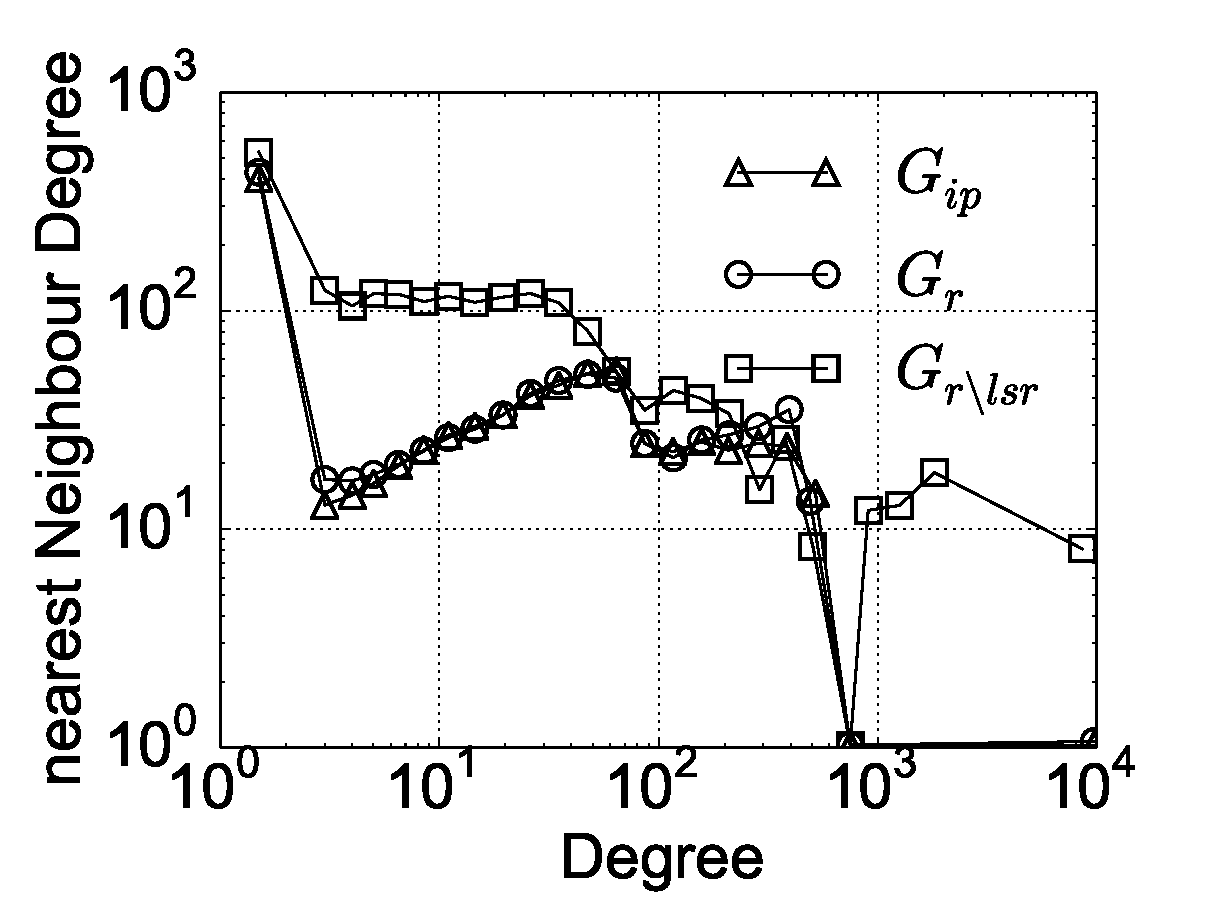
\includegraphics[width=2.2in]{NearestNeighbor}
\label{fig_metrics_c}}
\caption{ Dataset Metrics}
\label{fig_metrics}
\end{figure*}

Because part of our works focus on signature validation, we developed our own measurement tool in order to get \textit{qttl} and \textit{u-turn} signatures. We use \textit{conexdata explorer} [REF] software which is responsible to manage exploration through \textit{Planet Lab} Infrastructure. We choose 100 vantage point, selected randomly from the available set of Planet Lab Nodes. Additionally we selected 1M of targets IP address uniformly distributed over each VP. To achieve uniformity in target selection we used data provided by MaxMind\index{\url{www.maxmind.com}}. In this way, we choose a number of destinations according to the number of subnets assigned by the Regional Internet Registry to each region.

Our software use ICMP-Paris probes in order to avoid load balancing issues in the forwarding path. To get the \textit{u-turn} signature, we send a \textit{ping} to each hop revealed by traceroute. We sent six ICMP-echo packets from the same monitor. Six ICMP-echo responses allows us to infer with $95\%$ confidence if there is a single return path length and therefore reduce measurement error caused by a reverse path containing load-balanced segments of different lengths \cite{BRICE07}.

Finally, for better develop a realistic dataset, we build a router level topology. We resolve alias resolution issues using MIDAR. We found that $ \%$ of the discovered IP interfaces had at least one alias. IP level topology and router level topology (after alias resolution process) had similar characteristics as was expected. The main features related to our dataset are described in figure \ref{fig_metrics}.

To match the set of IP interfaces discovered to their respective Autonomus System, we use the RouteViews Dataset provided by CAIDA. 

Our experiment discovered around 260K IP interfaces and 520K links. Additionally we found MPLS tunnels on  $44\%$ of the traceroutes. The amount of explicit tunnels is highly superior to implicit tunnels. We discovered explicit tunnels on $34\%$ of traceroutes and at least one implicit tunnel on $16\%$. Surprisingly we found more implicit tunnels revealed trought \textit{u-turn} signature ($12\%$) rather than \textit{qttl} signature ($4\%$). We discuss these results in the next sections. Finally, we did not found opaque tunnels.


\section{MPLS signatures validation}

In this section we describe the used methodology to validate the MPLS signatures revealed by traceroutes. As we described previously, the RFC9450 and \textit{qttl} signature are fingerprints that occurs just on MPLS behaviour, while \textit{uturn} could be related with issues not related with MPLS such as load balancing. Thereby e mainly focus on test the \textit{u-turn} signatures. 

If the RFC 4950 is not implemented in the \textit{LSRs}, the only way to reveal an MPLS tunnel is trough \textit{qttl} or \textit{u-turn} signatures. Both of them are directly related with the position of MPLS within the tunnel.  

\begin{itemize}
\item[i] \textit{qttl} value refers to the \textit{TTL} of ICMP-\textit{echo} message when it enters to the MPLS  tunnel. A quoted \textit{TTL} of $n$ in the incoming ICMP-\textit{time-exceeded} reply means that the sent probe expired $n$ hops later to ingress to the \textit{LSP}. In this way, we can say that a \textit{LSR} that replies with $qttl=n$ appears  in the $n$ position of MPLS tunnel.

\item[ii] The \textit{u-turn} signature  relay on the difference in the incoming \textit{TTL} ICMP-\textit{time-exceeded} and \textit{TTL} ICMP-\textit{echo-reply}, indeed  $u-turn= TTL_{echo-reply}-TTL_{time-exceeded}$. The expected \textit{u-turn} value is in the form $[2L$, $2L-2$, $2L-4$, $...$, $2]$ where $L$ corresponds to the tunnel Length and the array position corresponds to the \textit{LSR} position within the MPLS tunnel.
\end{itemize}

%Figura u-turn
\begin{figure*}[!t]
\centering
\subfloat[Tunnel Length Distribution]{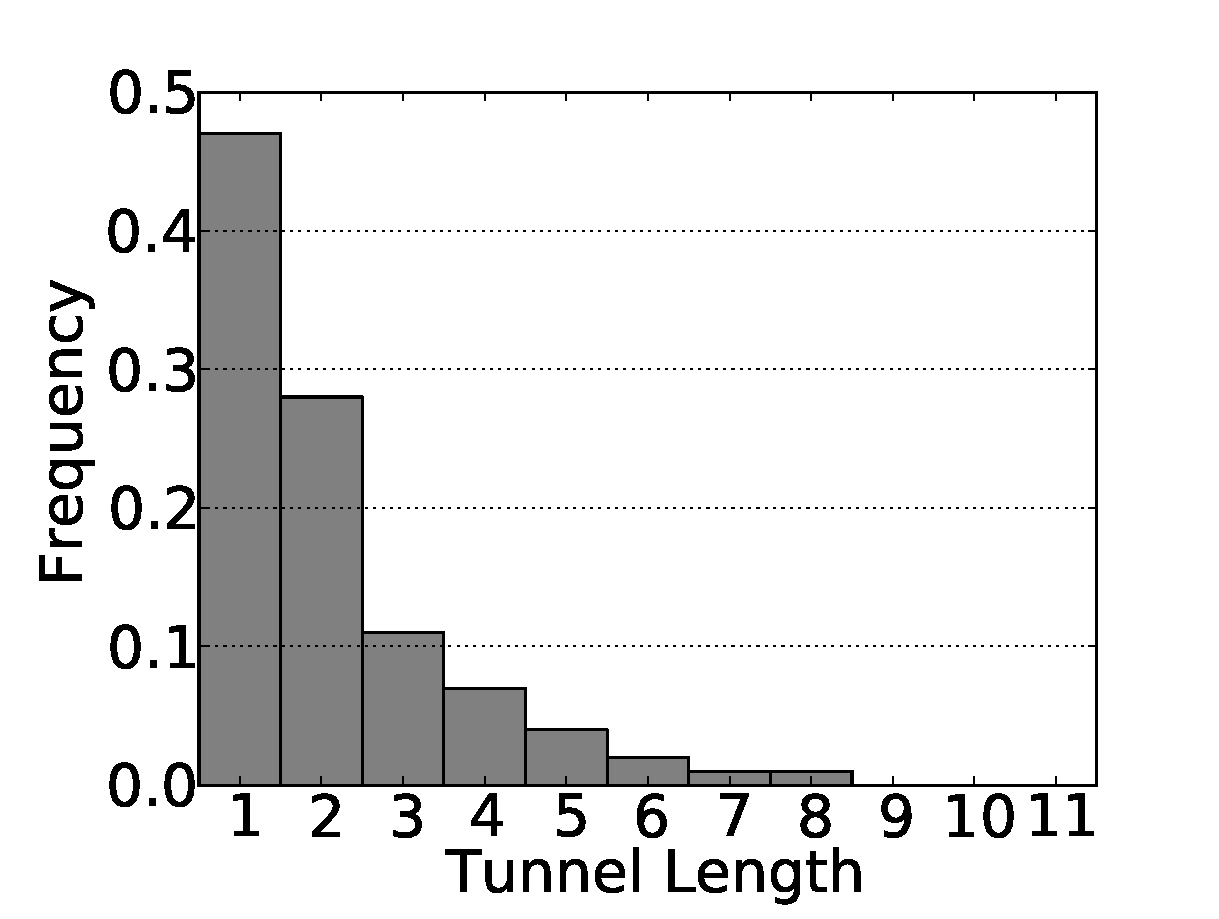
\includegraphics[width=2.5in]{hist_length}
\label{hist_length}}
\hfil
\subfloat[\textit{qttl} and $n$-position comparison]{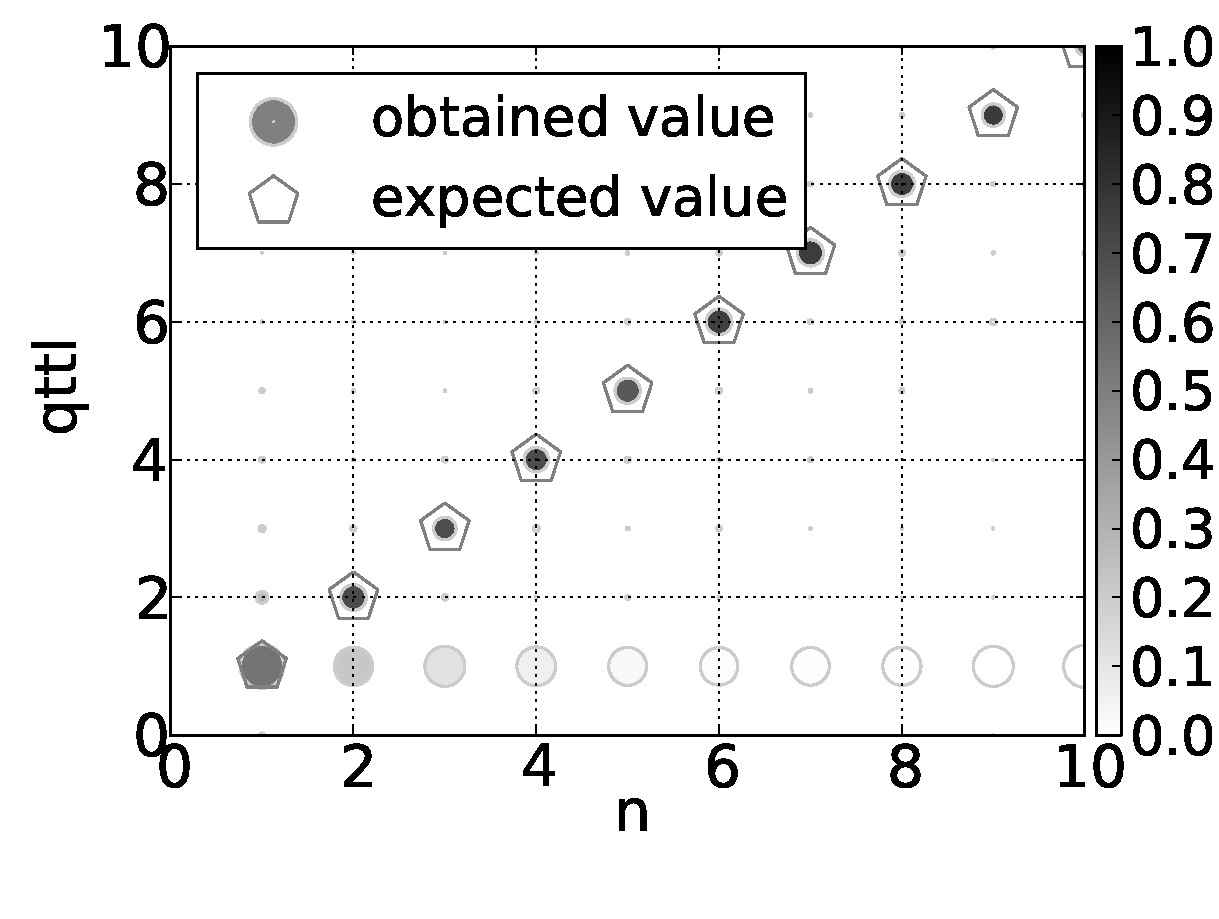
\includegraphics[width=2.5in]{n_vs_qttl}
\label{n_vs_qttl}}
\hfil
\subfloat[ \textit{u-turn} on \textit{LSRs} with no other signature was found ]{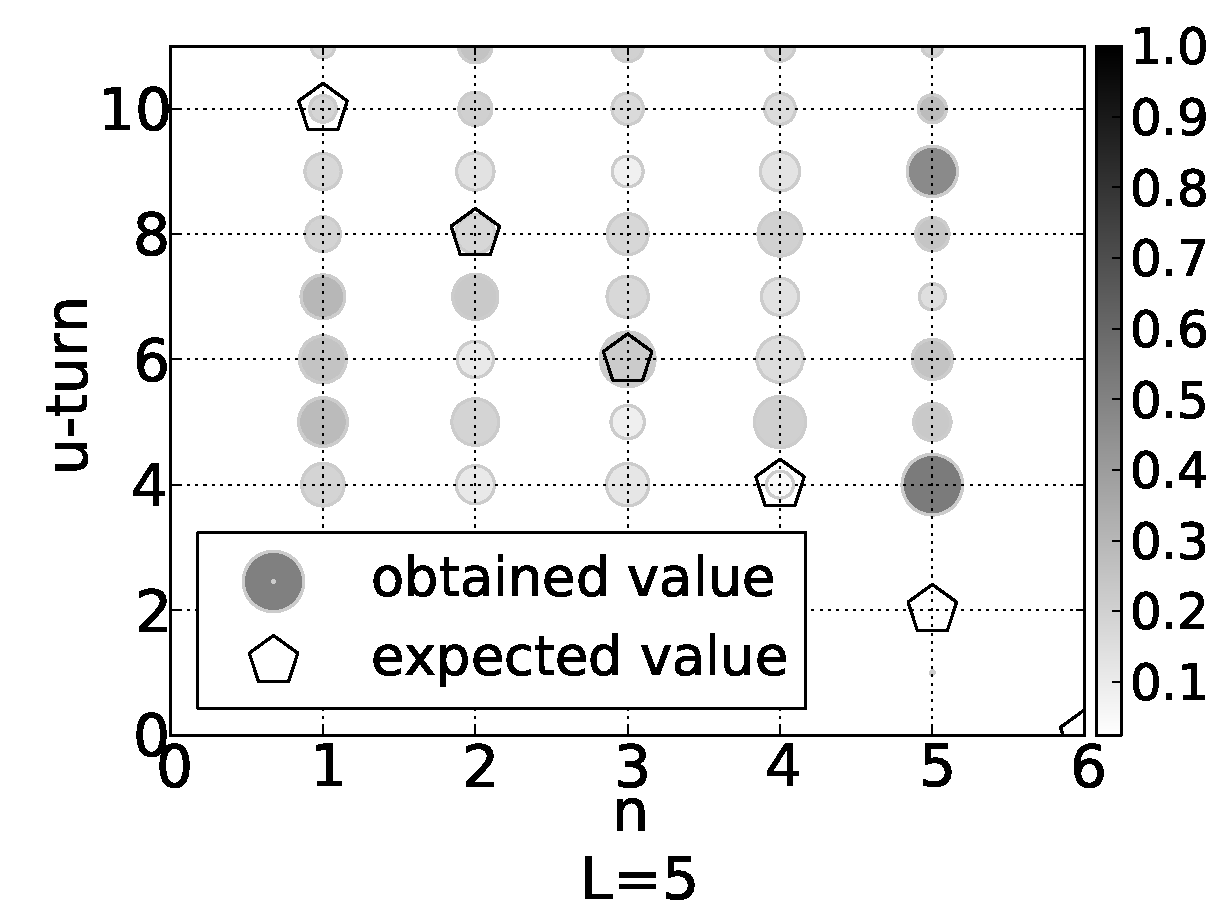
\includegraphics[width=2.5in]{n_vs_uturn_L5}%
\label{fig_uturn_a}}
\hfil
\subfloat[\textit{u-turn} on \textit{LSRs} revealed through RFC4950 and \textit{qttl}]{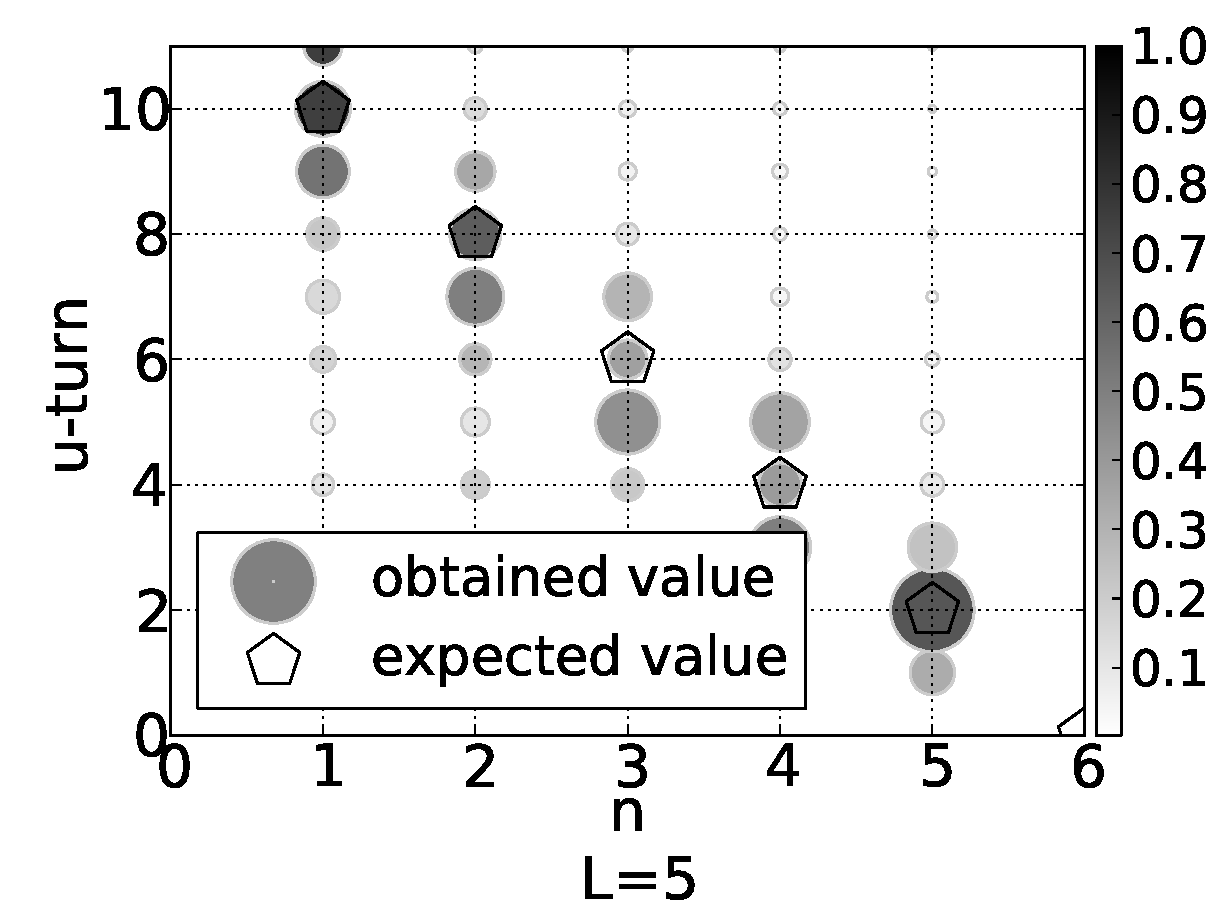
\includegraphics[width=2.5in]{n_vs_uturn_L5_exp}%
\label{fig_uturn_b}}
\caption{\textbf{.Comparison between obtained and expected values for \textit{qttl} and \textit{uturn} signatures}. The circle size in each circle is related with the frequency of \textit{u-turn} value founded regard each $n$-position. The transparency of the figure is related with the frequency of the  $n$-position regard each \textit{u-turn} value}
\label{fig_signatures}
\end{figure*}

%\begin{figure*}[!t]
%\centering
%\subfloat[Case I]{\includegraphics[width=2.5in]{box}%
%\label{fig_first_case}}
%\hfil
%\subfloat[Case II]{\includegraphics[width=2.5in]{box}%
%\label{fig_second_case}}
%\caption{Simulation results for the network.}
%\label{fig_sim}
%\end{figure*}


Our signature validation relays on the hypothesis that the MPLS position match with the $n$-position  which an \textit{LSR} is revealed by traceroute. Indeed we use a paris-traceroute based tool in order to sure that the probes follow the same path. In order to validate our hypotheses we first test it in explicit and implicit tunnels. Thereby we remove the bias caused by possible false \textit{u-turn} deltas. The \textit{qttl} value should to match with $n$-position, i.e., $qttl=n$. In order to test it, we first test the hypothesis to know the error generated by our assumption. Then, once it  was proved  we use $n$-position as a reference value to test the \textit{u-turn} signature. 

We compare the \textit{qttl} value and their respective position that the traceroute reveal to \textit{LSR} within the MPLS tunnel (if any). The obtained results are showing in figure \ref{n_vs_qttl}. We noticed that \textit{qttl} signature highly match with the $n$-position i.e., $qttl=n$.  A small bias occurs due to the limitation in our method to reveal the first \textit{LSRs} in the tunnel if it does not implement the RFC 4950 i.e., If the RFC 4950 is not implemented, the first LSR revealed by traceroute within the tunnel  ($n=1$) could correspond to a \textit{LSR} with $qttl>n$. A second small deviation occurs due to possible load balancer inference in the follow path. In this case, the traceroute probes follow paths with different lengths before to reach the MPLS tunnel. Therefore different traceroute probes (with different initial \textit{TTL} ) entered to the MPLS tunnel with the same TTL value. This issue produce that the same \textit{qttl} value were revealed in different $n$-positions. Finally, we noticed that in some cases the \textit{qttl} always remains at 1 for all positions. We think that this issue occurs because some routers update the $TTL_{ip}$ to one in the expired packet instead of keeping it unchanged. We found that in $58\%$ of the cases, the $n$-position match with the \textit{qttl} value, in $36,3\%$ of cases the \textit{qttl} signature is not present and always $qttl=1$, and finally just a $6,7\%$ of the cases presented some bias around the expected value.

Once we noticed that the \textit{qttl} value match with the $n$-position, we use this position as a reference value to validate the \textit{u-turn} signature. In this case, the expected value should to be $u-turn=2(L-(n-1))$ where $n$ is the position of the LSR within the tunnel and $L$ is the tunnel length. Because \textit{u-turn} is commonly present in almost \textit{LSRs}, first we test it in MPLS tunnels  where other signatures were found i.e., \textit{LSRs} revealed through RFC 4950 implementation (explicit tunnels) and \textit{qtll} signatures. Secondly we test it on \textit{LSRs} where \textit{u-turn} was the only signature that allows to reveal the MPLS tunnel. We use a filter ($u-turn>3$) to avoid false isolated \textit{u-turn} deltas. Some results are showed in figures \ref{fig_uturn_a}, \ref{fig_uturn_b} . We compare the expected value and the obtained value using a scatter plot where we can distinguish the amount of signatures biased. We found the same results for different tunnel lengths. We noticed that on \textit{LSRs} revealed through RFC 4950 implementation and \textit{qtll} signatures, the $60\%$ of obtained \textit{u-turn} values match with the expected values. However when we compare the results in \textit{LSRs} where no other signature exists (therefore where the \textit{u-turn} signatures are really useful), the obtained \textit{u-turn} signature just match in $25\%$  so we can conclude that the \textit{LSRs} revealed through \textit{u-turn} signatures are highly overestimated. Mainly because MPLS tunnels are not the only behaviour that causes the \textit{u-turn} delta  and it is also related with load balancing issues. Indeed, available tools used to avoid load balancing issues are based on keep constant the first 32 bits of the IP \textit{payload} \cite{BRICE06}. In the case of ICMP messages, this fields are \textit{Type}, \textit{Code} and \textit{Checksum}. By definition, \textit{u-turn} signature is based on two kinds of ICMP message: ICMP \textit{reply}-Code 11 and ICMP \textit{time exceeded}-Code 0. Thereby, because the different codes values related with each ICMP message, there is no way to sure that the \textit{u-turn} value is caused just by MPLS tunnels.


\section{\textit{LSRs} and MPLS clouds}

\subsection{Methodolody}

For the best of our acknowledge, MPLS architecture on Internet Topology has not been yet studied. In this way, we focus our attention on study some properties of \textit{LSRs} and \textit{MPLS clouds}. The \textit{LSRs} refers to routers with MPLS capabilities and \textit{MPLS clouds} refer to networks of \textit{LSRs} linked through MPLS tunnels. 

Generally speaking, we propose a study  in order to better understand the interaction inward and outward between MPLS networks and non MPLS networks (IP level).

For our purposes , following  we define some some basic terminology for the remains of the work.  

\textbf{IP level Graph}. IP level graph $G_{ip}=(V_{ip}, E_{ip})$, where $V_{ip}$ is the IP address discovered in our exploration and $E_{ip}$ is the set of the links founded trough traceroute. 

\textbf{Router Level Graph}. Graph obtained after apply the Alias Resolution Process using MIDAR over the set of IP address $V_{ip}$ . As a result we get the graph $G_{r}=(V_{r}, E_{r})$, where $V_{r}$ is the set of routers where we found at least one IP address and $E_{r}$ is the set of all the links founded between any pair of routers.

\textbf{MPLS IP level Graph}. IP level subgraph build by IP interfaces where we discovered at least one MPLS tunnel. Formally, $G^{mpls}_{ip}=(V^{mpls}_{ip}, E^{mpls}_{ip})$, where  $V^{mpls}_{ip}$ is the set of IP address  belonging to an MPLS tunnel and  $ E^{mpls}_{ip}$ is the set of all \textit{mpls links} $(v^{mpls(a)}_{ip}, v^{mpls(b)}_{ip})$ such as $v^{mpls(a)}_{ip}$ and $v^{mpls(b)}_{ip}$ $\in V^{mpls}_{ip}$.


\textbf{MPLS router level Graph}. Router level subgraph builded by routers where we find at least one MPLS interfaces. Formally, $G^{mpls}_{lsr}=(V^{mpls}_{lsr}, E^{mpls}_{lsr})$, where  $V^{mpls}_{lsr}$ is the set of routers where we founded at least one IP address belonging to an MPLS tunnel and  $E^{mpls}_{lsr}$ is the set of all \textit{mpls links} $(v^{mpls(a)}_{lsr}, v^{mpls(b)}_{lsr})$ such as $v^{mpls(a)}_{lsr}$ and  $v^{mpls(b)}_{lsr}$  $\in V^{mpls}_{lsr}$.

\textbf{Induced Graph by nodes belonging to the same AS}. We define the graphs $G^{(as)}_{ip}$, $G^{(as)}_{r}$, $G^{mpls(as)}_{ip}$ and $G^{mpls(as)}_{lsr}$ as the induced graphs of  $G_{ip}$, $G_{r}$, $G^{mpls}_{ip}$ and $G^{mpls}_{lsr}$ respectively, such as the vertexes of the Graphs belongs to the same Autonomous System $as$. For router level topology, where the IP interfaces could belong to different ASs, we discard the interfaces that do not belong to $as$.


\textbf{MPLS Clouds}. We define two levels of MPLS clouds: IP and router level clouds. An IP level MPLS cloud $C^{mpls(i)}_{ip}$ is a connected component $i$ of $G^{mpls(as)}_{ip}$ . A router level MPLS cloud $C^{mpls(i)}_{lsr}$ is a connected component $i$ of $G^{mpls(as)}_{lsr}$. In simple words, we define a \textit{MPLS cloud} as a connected component of \textit{LSRs} whose interfaces belonging to the same Autonomous System. One Autonomous system could to have several \textit{mpls clouds}

\textbf{MPLS Cloud level Graph}. We define an MPLS Cloud level Graph as an hybrid IP level graph $G_{ip\backslash lsr}$  or an hybrid router level graph $G_{r\backslash lsr}$  where all the \textit{MPLS Clouds} were contracted to a single node while IP interfaces  and  routers remains unchanged. Finally, we called $G^{as}_{ip\backslash lsr}$ and $G^{as}_{r\backslash lsr}$ to the induced subgraphs of $G_{ip\backslash lsr}$ and $G_{r\backslash lsr}$ respectively, such as each vertex of the graphs are in the Autonomous System $as$. Broadly speaking, an \textit{MPLS Cloud level Graph} refers to a graph where all MPLS clouds are treated as a single node. In this way, we can study how non MPLS interfaces and non MPLS routers interact with MPLS networks.


\subsection{MPLS on Internet Topology} 

\begin{figure}[!t]
\centering
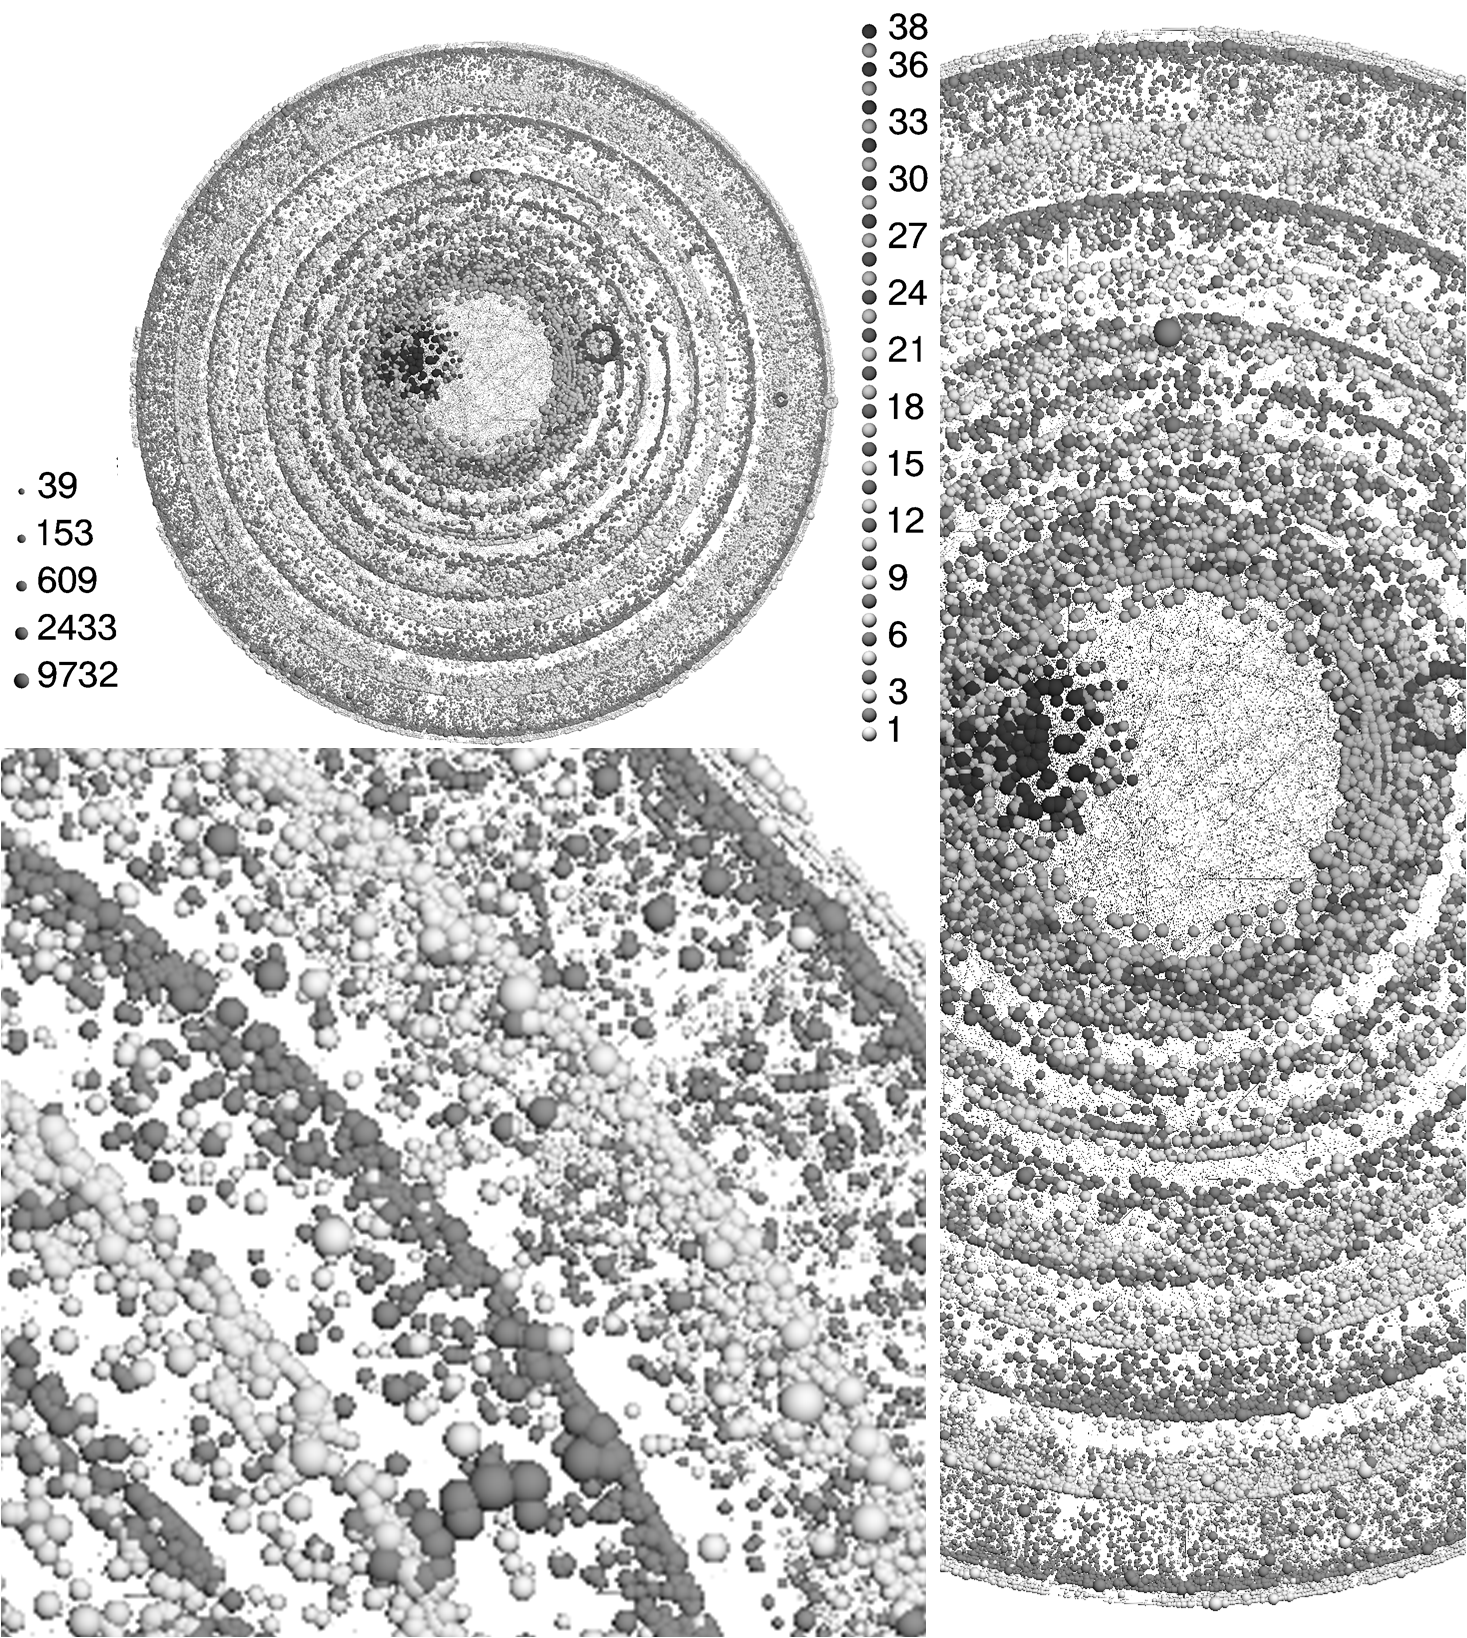
\includegraphics[width=3in]{Routers}
\caption{$k$-core visualization of router level topology $G_{r}=(V_{r}, E_{r})$ }
\label{fig_k_core_routers}
\end{figure}

Mainly, we based on $k$-core decomposition in order to study the fingerprints printed by \textit{LSRs} and \textit{MPLS clouds} on Internet topology, as well as some topological properties of MPLS networks. 

First we analyse the graphs $G_{ip}$ and $G_{r}$ in order to know if there is some strong difference between their structure and properties. As was expected we noticed that the router level topology has strong clustering coefficient than ip level topology. This fact occurs due to the join of ip interfaces into single routers. However, the structure of both topologies are identical. We also compared this topologies using $k$-core decomposition and given that we did not notice any meaningful difference between them and because router level topology are more approached to a realistic Internet behaviour , we selected router level topologies based for the remain of the analysis.

Figure \ref{fig_k_core_routers} shows the $k$-core visualization of $G_{r}$. In the center is located the shell index with the $k_{max}-core$ and the rest of the shells are located concentrically around it. On the right is a gray scale with the shell index $c_i$ and left is a node degree scale represented by the size of each one. We see that all the shells index are highly populated and that the node degree is not related with the shell index i.e., there is many routers with high degree in the outer shells. In order to locate \textit{LSRs}-routers with mpls capabilities into the shells index, we painted in black the  \textit{non MPLS capable routers} and in gray color the \textit{LSRs}. The results are showed in figure \ref{fig_k_core_LSR}. For the sake of the visualization we do not include the shell index and degree scale. We noticed that the \textit{LSRs} are distributed around the different shells of Internet but  lightly tends to concentrate with more density nearby to the core. Additionally, we apply the same concept for the MPLS cloud level graph $G_{r\backslash lsr}$. The figure \ref{fig_k_core_MPLS} shows the getting results. We distinguish the MPLS clouds with gray color. In this case, the MPLS clouds  are also spread out on the Internet, indeed we see some well defined gray nodes on the periphery. However MPLS clouds shows a stronger tendency to concentrate it near to the core.

\subsection{MPLS on Autonomous Systems}

Although the previous results give us a general overview around MPLS deployment, we believe that the study of MPLS structure requires a zoom in on each MPLS cloud or at least within each Autonomous System. Indeed, we found that around $89.9\%$ of \textit{mpls links} are intra\textit{AS}).  Thereby in order to get a zoom on MPLS architecture we selected the principal \textit{ASs} we reveal. We choose the top ten of \textit{ASs} according to the amount of  links discovered. In order to avoid bias related with AS not well explored,  we discard those where we found less than five hundred of \textit{mpls links}. Additionally we identified the \textit{mpls links} according to the kind of tunnel. The summary of the top \textit{AS} is showed in the figure \ref{top_as}. We noticed that the ratio $r_{mpls}$ between \textit{mpls links} and the total amount of links discovered by \textit{AS} is greater when more explicit \textit{mpls links} have been discovered. Interestingly, we also see that the \textit{ASs} with more links discovered have the lowest ratio $r_{mpls}$. This fact suggests that exists a high amount of invisible tunnels in this Autonomous System.

\begin{figure*}[!t]
\centering
\subfloat[]{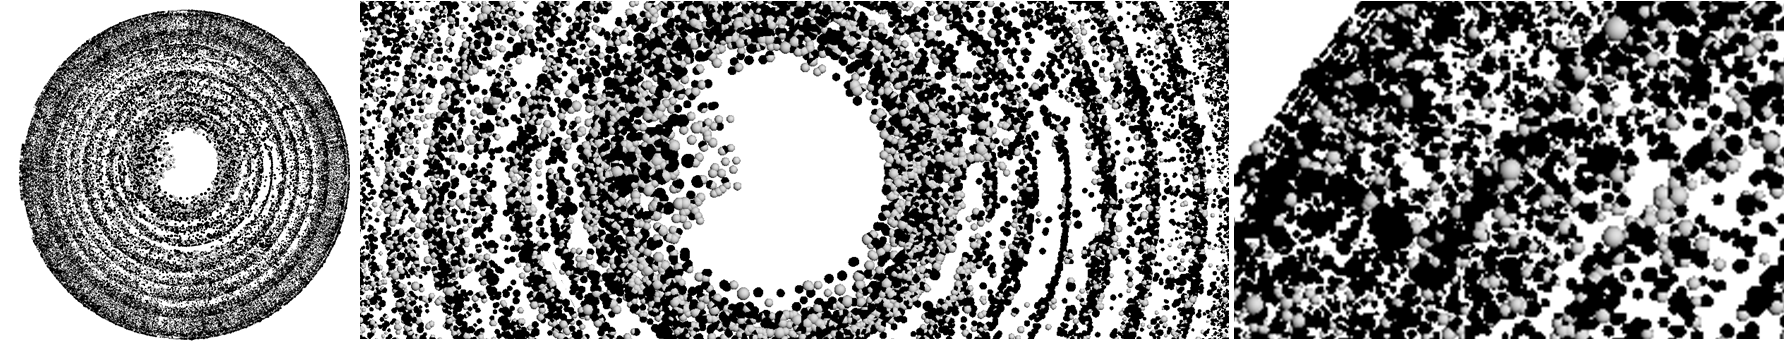
\includegraphics[width=6in]{LSR}%
\label{fig_k_core_LSR}}
\hfil
\subfloat[]{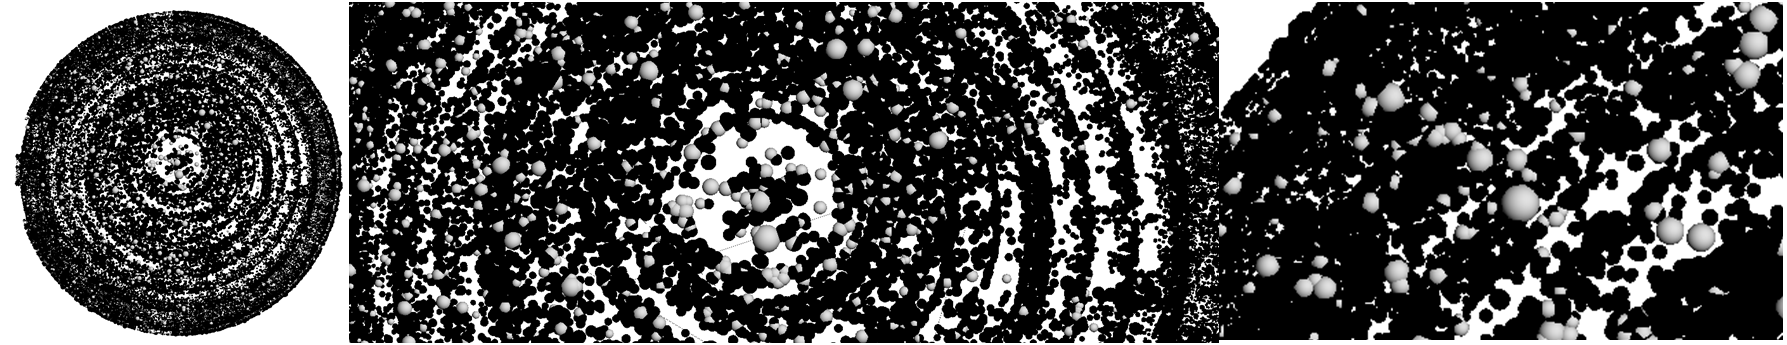
\includegraphics[width=6in]{MPLS}%
\label{fig_k_core_MPLS}}
\caption{ (a) $k$-core visualization of router level topology  $G_{r}=(V_{r}, E_{r})$. Black nodes refer to non MPLS capable routers and gray nodes refer no LSRs. (b) $k$-core visualization of MPLS cloud level topology  $G_{r\backslash lsr}$. Black nodes refer to non MPLS capable routers and gray nodes refer to MPLS clouds}
\label{fig_kcore_overview}
\end{figure*}



\begin{figure}[!t]
\centering
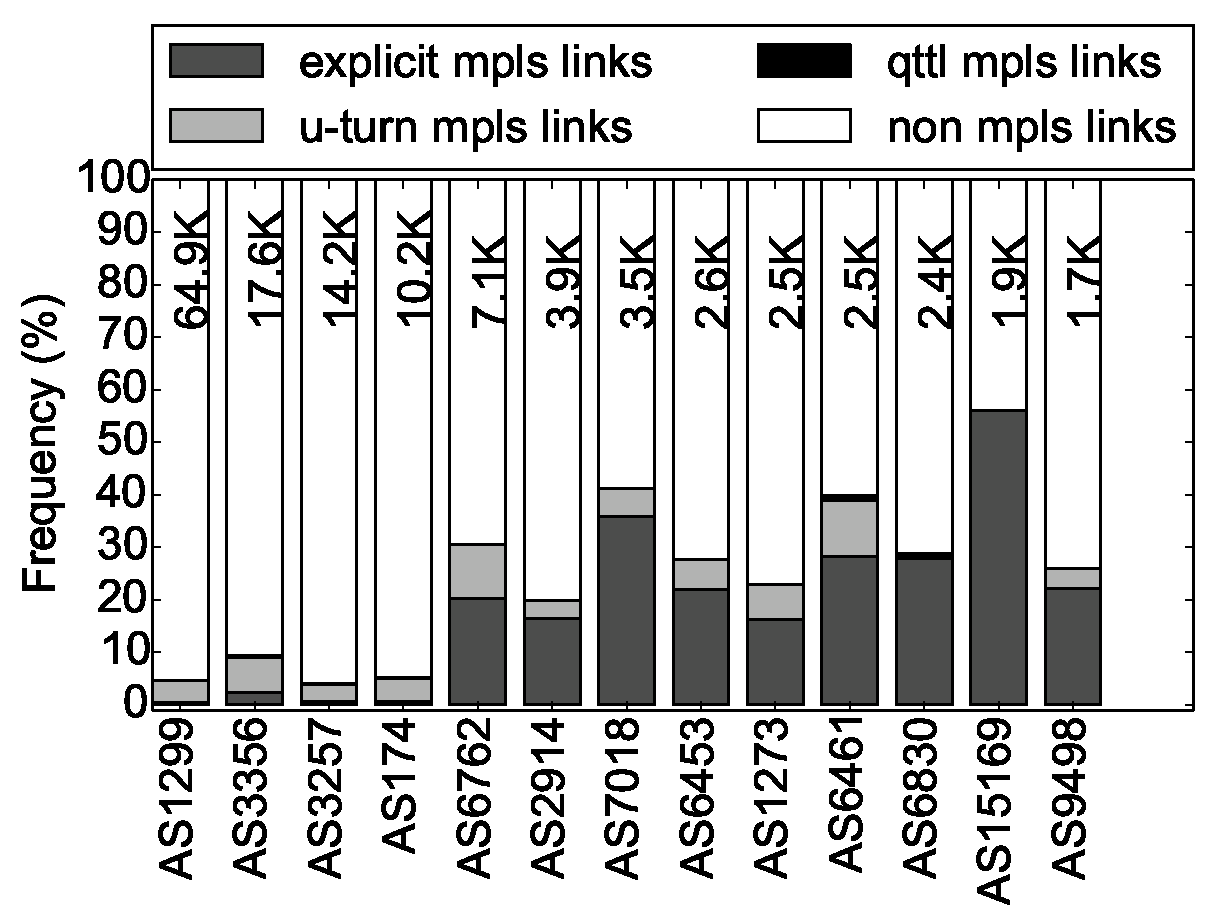
\includegraphics[width=3in]{TOP_AS}
% where an .eps filename suffix will be assumed under latex, 
% and a .pdf suffix will be assumed for pdflatex; or what has been declared
% via \DeclareGraphicsExtensions.
\caption{\textbf{Top of Autonomous System with most links discovered}}
\label{top_as}
\end{figure}

In this section, we study the graphs $G^{as}_{r}$ and $G^{as}_{r\backslash lsr}$. We applied the same analysis based on $k$-core decomposition used previously.  Regarding the graph $G^{as}_{r}$, we find that almost of \textit{LSRs} tends to locate in the vicinity of the cores, similar to that observed on $G_{r}$ in the previous section. However, the most remarkable observation around the analysis of MPLS per \textit{ASs} occurs regarding the graph $G^{as}_{r\backslash lsr}$: $k$-core visualization highly differs on those \textit{ASs} where prevails explicit tunnels in comparison with those where high percentage of \textit{u-turn} coverage i.e., \textit{ASs} that have more than $1/3$ of tunnels revealed by \textit{u-turn} signatures. The figures \ref{fig_cloud_mpls_174}, \ref{fig_cloud_mpls_1299}, \ref{fig_cloud_mpls_6762} shows this observation. The figures show visualization based on $k$-core decomposition for the graphs $G^{as}_{r\backslash lsr}$  for the autonomous system AS174, AS1299 and AS6762. The \textit{MPLS clouds} located in this autonomous systems (represented as gray nodes) are spread out over the different shells index. This $k$-core structure are similar in our top four of \textit{ASs}, where \textit{u-turn} signature was majority discovered i.e., between $30\%$ and  $80\%$ over  the total of \textit{mpls links}. However, for the rest of \textit{ASs} where prevails explicit tunnels, we found a $k$-core structure highly different.  In this cases,  the \textit{ASs} seems to have few and well defined MPLS clouds, mainly belonging to the maximum $k_{max}$-core. Some examples of this $k$-core structure are showed on figures \ref{fig_cloud_mpls_7018}, \ref{fig_cloud_mpls_1273} and \ref{fig_cloud_mpls_2914}. The same result was noticed in the rest of top \textit{ASs}. This observation suggest that exists a great number of\textit{MPLS} links non revealed in the top four of \textit{ASs}, therefore  the \textit{LSRs} discovered can not build large \textit{MPLS} clouds so they are thoroughly spread out. Additionally, because \textit{u-turn} signatures are overestimated, as we showed previously, there are several false \textit{LSRs} spread out over the shell indexes, adding false MPLS clouds.

Another remarkable characteristic  relays on the fact that the degree reached by the MPLS clouds is considerably high in comparison with the network size \textit{ASs}of each . Indeed, with exception of AS174, the rest of top \textit{ASs } suggest that more than $50\%$ of non mpls routers connects to at least one \textit{LSR}. Even the outer shells of the $k$-core decomposition are linked directly with the MPLS clouds located in the core. 

%Figura u-turn
\begin{figure*}[!t]
\centering
\subfloat[AS174]{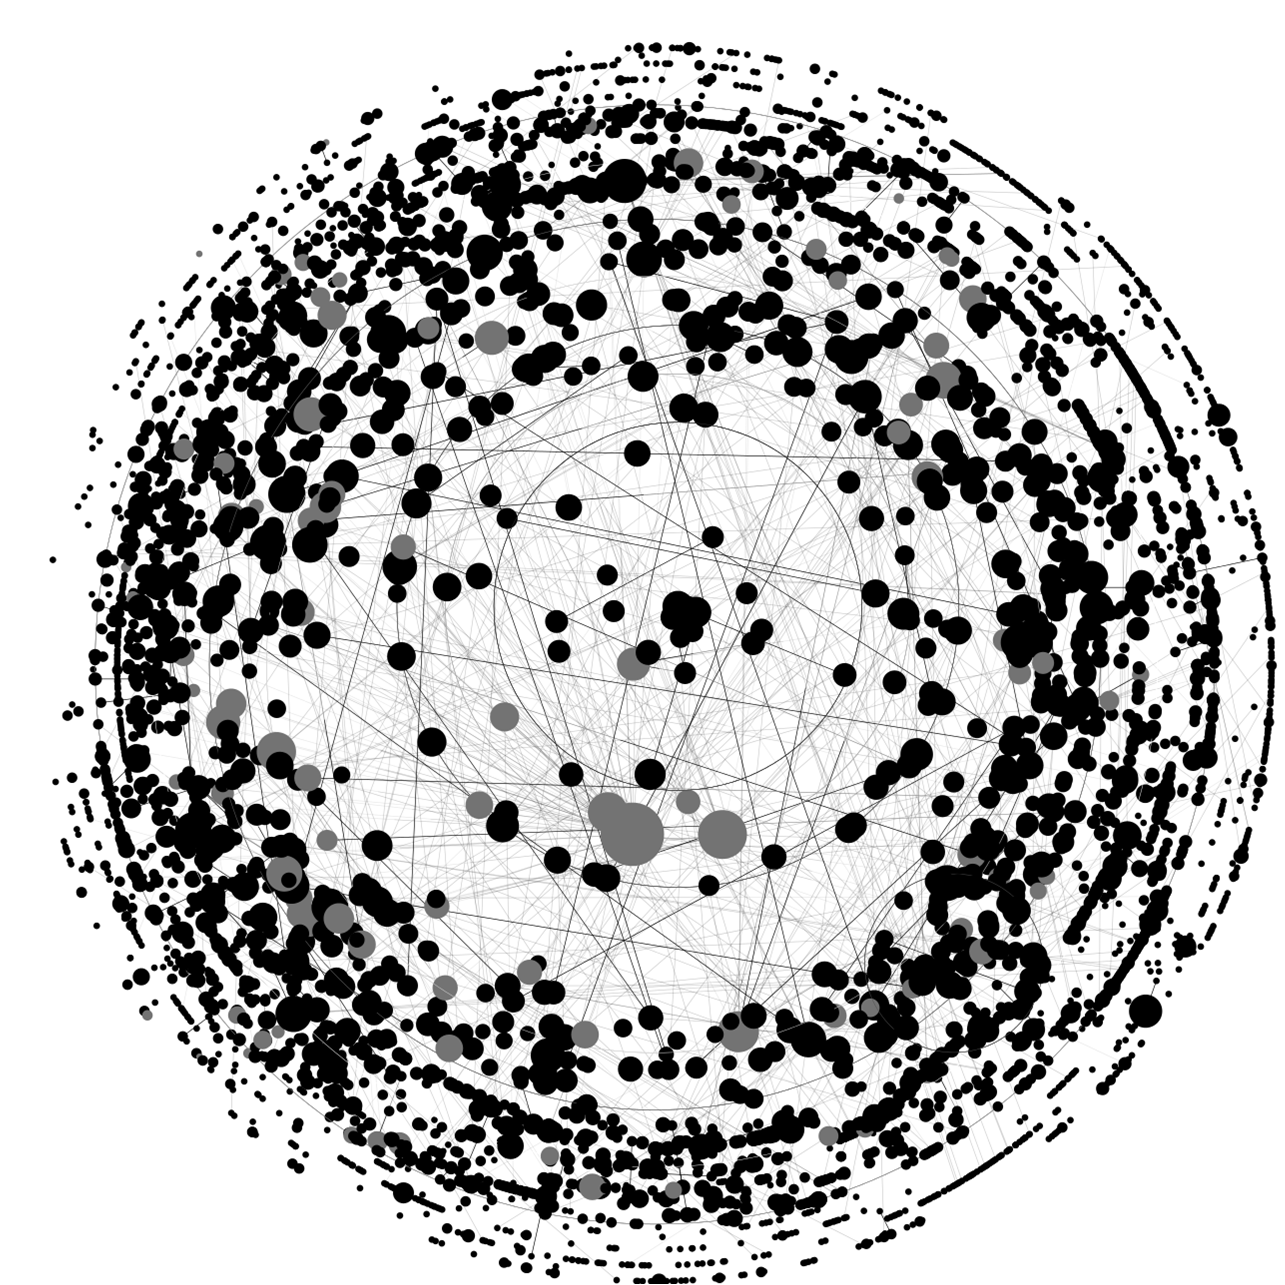
\includegraphics[width=2in]{174}%
\label{fig_cloud_mpls_174}}
\hfil
\subfloat[AS1299]{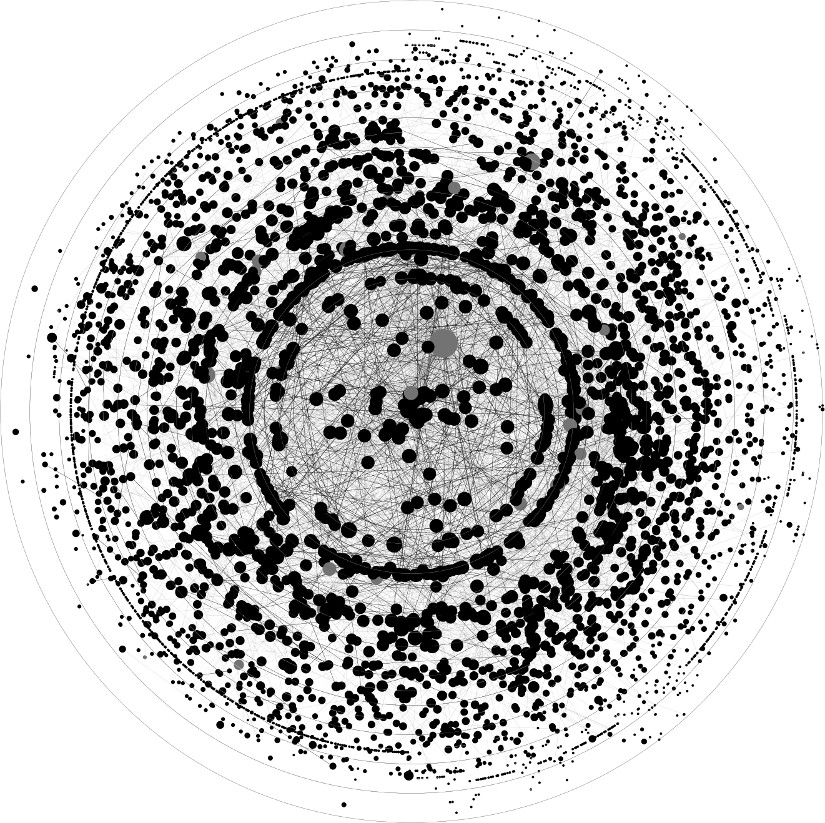
\includegraphics[width=2in]{1299}%
\label{fig_cloud_mpls_1299}}
\hfil
\subfloat[AS6762]{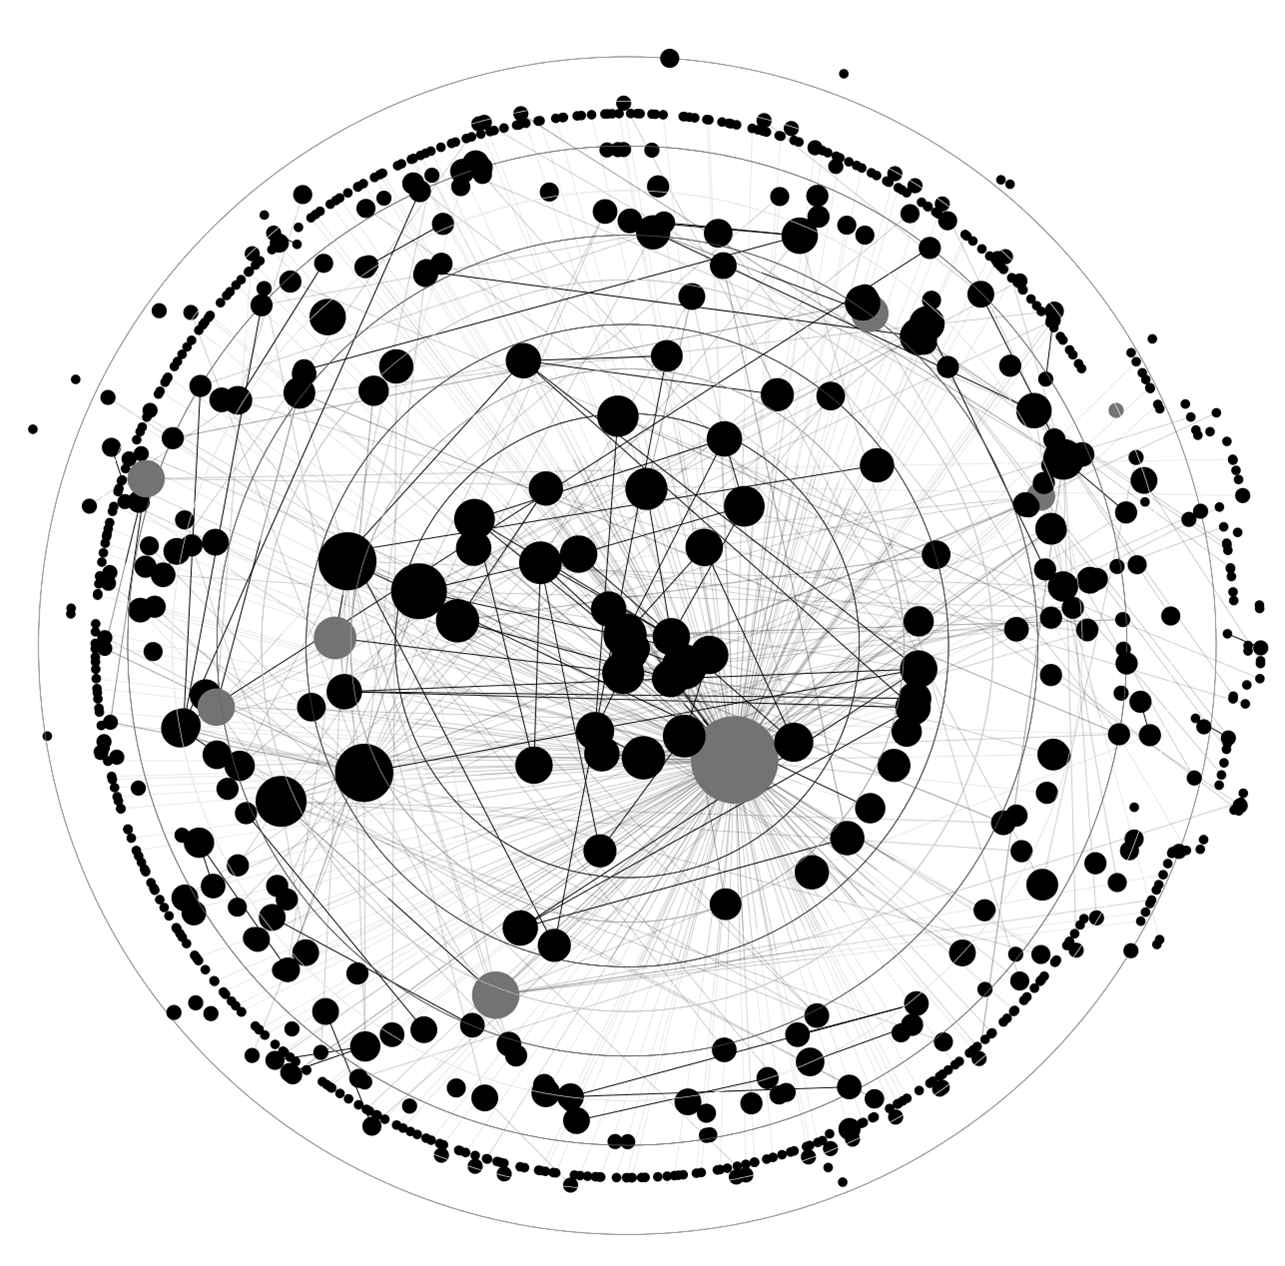
\includegraphics[width=2in]{6762}%
\label{fig_cloud_mpls_6762}}
\hfil
\subfloat[AS7018]{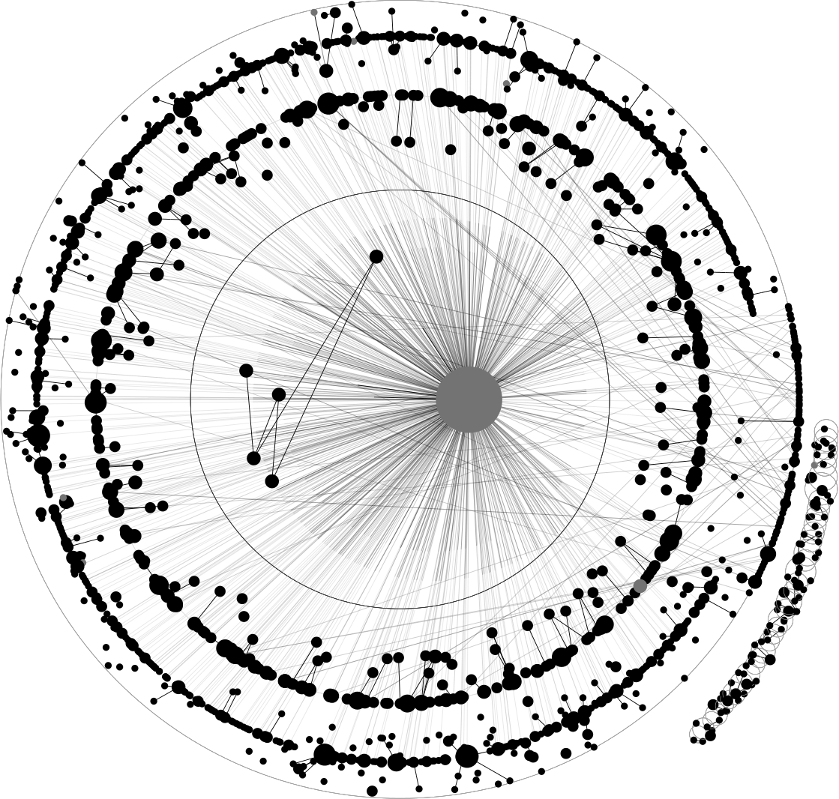
\includegraphics[width=2in]{7018}%
\label{fig_cloud_mpls_7018}}
\hfil
\subfloat[ AS1273]{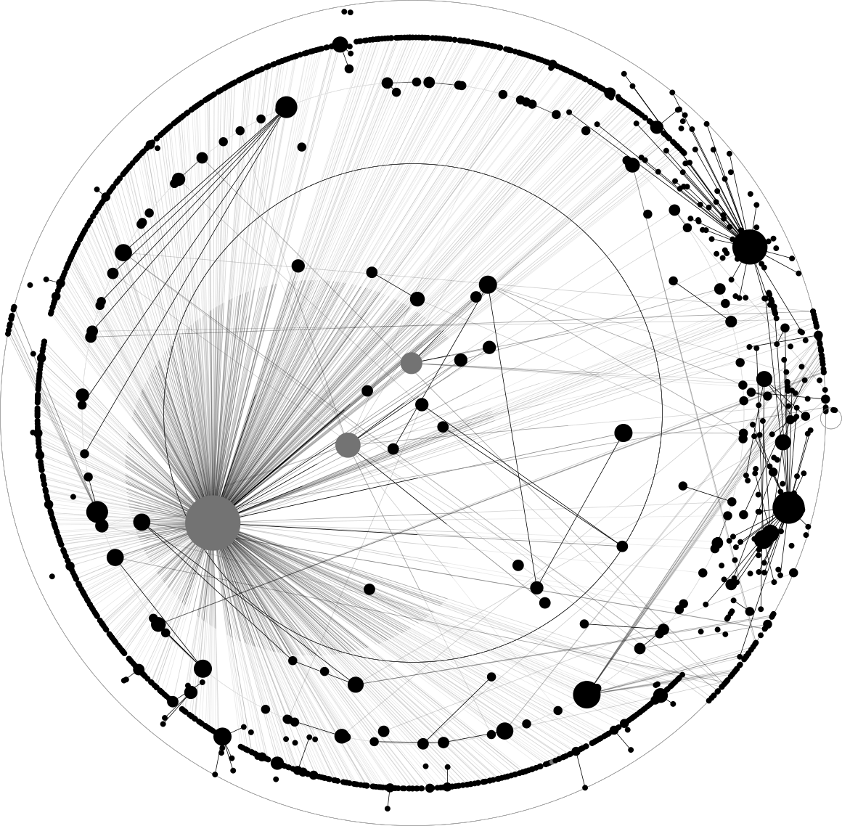
\includegraphics[width=2in]{1273}%
\label{fig_cloud_mpls_1273}}
\hfil
\subfloat[AS2914]{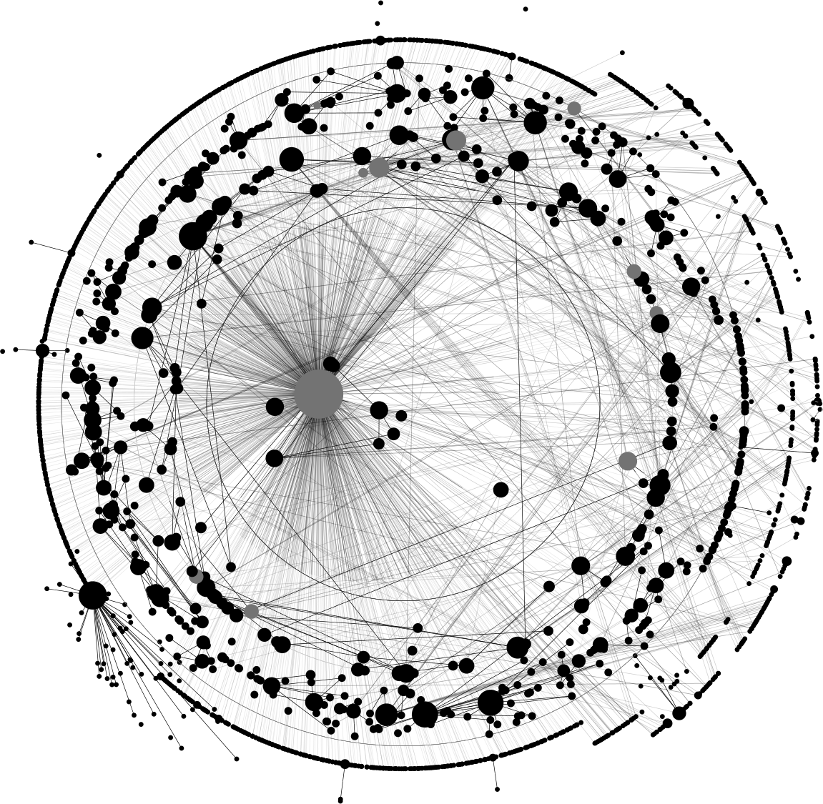
\includegraphics[width=2in]{2914}%
\label{fig_cloud_mpls_2914}}
\caption{$k$-core visualization of MPLS cloud level topology by \textit{ASs} $G^{as}_{ip\backslash lsr}$.}
\label{fig_cloud_mpls}
\end{figure*}

\section{Further Work}

\section{Conclusions}



%\section{Introduction}
% no \IEEEPARstart
%This demo file is intended to serve as a ``starter file''
%for IEEE conference papers produced under \LaTeX\ using
%IEEEtran.cls version 1.8b and later.
% You must have at least 2 lines in the paragraph with the drop letter
% (should never be an issue)
%I wish you the best of success.

%\hfill mds
 
%\hfill August 26, 2015

%\subsection{Subsection Heading Here}
%Subsection text here.


%\subsubsection{Subsubsection Heading Here}
%Subsubsection text here.


% An example of a floating figure using the graphicx package.
% Note that \label must occur AFTER (or within) \caption.
% For figures, \caption should occur after the \includegraphics.
% Note that IEEEtran v1.7 and later has special internal code that
% is designed to preserve the operation of \label within \caption
% even when the captionsoff option is in effect. However, because
% of issues like this, it may be the safest practice to put all your
% \label just after \caption rather than within \caption{}.
%
% Reminder: the "draftcls" or "draftclsnofoot", not "draft", class
% option should be used if it is desired that the figures are to be
% displayed while in draft mode.
%
%\begin{figure}[!t]
%\centering
%\includegraphics[width=2.5in]{myfigure}
% where an .eps filename suffix will be assumed under latex, 
% and a .pdf suffix will be assumed for pdflatex; or what has been declared
% via \DeclareGraphicsExtensions.
%\caption{Simulation results for the network.}
%\label{fig_sim}
%\end{figure}

% Note that the IEEE typically puts floats only at the top, even when this
% results in a large percentage of a column being occupied by floats.


% An example of a double column floating figure using two subfigures.
% (The subfig.sty package must be loaded for this to work.)
% The subfigure \label commands are set within each subfloat command,
% and the \label for the overall figure must come after \caption.
% \hfil is used as a separator to get equal spacing.
% Watch out that the combined width of all the subfigures on a 
% line do not exceed the text width or a line break will occur.
%
%\begin{figure*}[!t]
%\centering
%\subfloat[Case I]{\includegraphics[width=2.5in]{box}%
%\label{fig_first_case}}
%\hfil
%\subfloat[Case II]{\includegraphics[width=2.5in]{box}%
%\label{fig_second_case}}
%\caption{Simulation results for the network.}
%\label{fig_sim}
%\end{figure*}
%
% Note that often IEEE papers with subfigures do not employ subfigure
% captions (using the optional argument to \subfloat[]), but instead will
% reference/describe all of them (a), (b), etc., within the main caption.
% Be aware that for subfig.sty to generate the (a), (b), etc., subfigure
% labels, the optional argument to \subfloat must be present. If a
% subcaption is not desired, just leave its contents blank,
% e.g., \subfloat[].


% An example of a floating table. Note that, for IEEE style tables, the
% \caption command should come BEFORE the table and, given that table
% captions serve much like titles, are usually capitalized except for words
% such as a, an, and, as, at, but, by, for, in, nor, of, on, or, the, to
% and up, which are usually not capitalized unless they are the first or
% last word of the caption. Table text will default to \footnotesize as
% the IEEE normally uses this smaller font for tables.
% The \label must come after \caption as always.
%
%\begin{table}[!t]
%% increase table row spacing, adjust to taste
%\renewcommand{\arraystretch}{1.3}
% if using array.sty, it might be a good idea to tweak the value of
% \extrarowheight as needed to properly center the text within the cells
%\caption{An Example of a Table}
%\label{table_example}
%\centering
%% Some packages, such as MDW tools, offer better commands for making tables
%% than the plain LaTeX2e tabular which is used here.
%\begin{tabular}{|c||c|}
%\hline
%One & Two\\
%\hline
%Three & Four\\
%\hline
%\end{tabular}
%\end{table}


% Note that the IEEE does not put floats in the very first column
% - or typically anywhere on the first page for that matter. Also,
% in-text middle ("here") positioning is typically not used, but it
% is allowed and encouraged for Computer Society conferences (but
% not Computer Society journals). Most IEEE journals/conferences use
% top floats exclusively. 
% Note that, LaTeX2e, unlike IEEE journals/conferences, places
% footnotes above bottom floats. This can be corrected via the
% \fnbelowfloat command of the stfloats package.




%\section{Conclusion}
%The conclusion goes here.




% conference papers do not normally have an appendix


% use section* for acknowledgment
%\section*{Acknowledgment}


%The authors would like to thank...





% trigger a \newpage just before the given reference
% number - used to balance the columns on the last page
% adjust value as needed - may need to be readjusted if
% the document is modified later
%\IEEEtriggeratref{8}
% The "triggered" command can be changed if desired:
%\IEEEtriggercmd{\enlargethispage{-5in}}

% references section

% can use a bibliography generated by BibTeX as a .bbl file
% BibTeX documentation can be easily obtained at:
% http://mirror.ctan.org/biblio/bibtex/contrib/doc/
% The IEEEtran BibTeX style support page is at:
% http://www.michaelshell.org/tex/ieeetran/bibtex/
%\bibliographystyle{IEEEtran}
% argument is your BibTeX string definitions and bibliography database(s)
%\bibliography{IEEEabrv,../bib/paper}
%
% <OR> manually copy in the resultant .bbl file
% set second argument of \begin to the number of references
% (used to reserve space for the reference number labels box)
%\begin{thebibliography}{1}

%\bibitem{IEEEhowto:kopka}
%H.~Kopka and P.~W. Daly, \emph{A Guide to \LaTeX}, 3rd~ed.\hskip 1em plus
%  0.5em minus 0.4em\relax Harlow, England: Addison-Wesley, 1999.

%\end{thebibliography}


\bibliographystyle{IEEEtran}
\bibliography{IEEEabrv,Bibliography}



% that's all folks
\end{document}


